% Options for packages loaded elsewhere
\PassOptionsToPackage{unicode}{hyperref}
\PassOptionsToPackage{hyphens}{url}

%=========
% BEAMER CLASS OPTIONS
%=========
\documentclass[%
  9pt,
  spanish, % Set language for babel
  ignorenonframetext,
  aspectratio=169, % Set aspect ratio (default: 16:9)
]{beamer}

% ==========
% MAIN PACKAGES
% ==========
\usepackage{tikz}
\usepackage{etoolbox}
\usepackage{setspace}

% Set the language
\usepackage[shorthands=off,%
main=spanish]{babel}

\usepackage{pgfpages}

% ==========
% CAPTIONS FOR FIGURES
% ==========
\setbeamertemplate{caption}[numbered]
\setbeamertemplate{caption label separator}{: }
\setbeamercolor{caption name}{fg=normal text.fg}
\beamertemplatenavigationsymbolsempty

% =========
% BEAMER OPTIONS
% =========

% Prevent slide breaks in the middle of a paragraph
\widowpenalties 1 10000
\raggedbottom

% Templates for slide section titles
% We need to design the 'part' slide, which is a special slide in beamer
\setbeamertemplate{part page}{
  \centering
  \begin{beamercolorbox}[sep=16pt,center]{part title}
    \usebeamerfont{part title}\insertpart\par
  \end{beamercolorbox}
}
\AtBeginPart{
  \frame{\partpage}
}

% Define the section and subsection slides
\setbeamertemplate{section page}{
  \centering
  \begin{beamercolorbox}[sep=12pt,center]{part title}
    {\usebeamerfont{section name}\usebeamercolor[fg]{section name}}
    {\usebeamerfont{section title}\insertsection\par}
  \end{beamercolorbox}
}
\AtBeginSubsection{
  \frame{\subsectionpage}
}


\usepackage{ifxetex,ifluatex}
\ifnum 0\ifxetex 1\fi\ifluatex 1\fi=0 % if pdftex
\usepackage[T1]{fontenc}
\usepackage[utf8]{inputenc}
\usepackage{textcomp} % provide euro and other symbols
\fi

% =========
% DEFAULT SLIDE DESIGN
% =========

% Sets the slide theme. Default: Berlin %
\usetheme{Berlin}
\makeatletter
\def\beamer@writeslidentry{\clearpage\beamer@notesactions}
\makeatother

% Slide text size
\setbeamersize{text margin left=3em, text margin right=3em}

\setlength{\emergencystretch}{3em} % prevent overfull lines

% Head Line (Section bar on the top of each slide)
\setbeamercolor{headline}{bg=main-color!50!black,fg=white}
\setbeamertemplate{headline}{%
  \begin{beamercolorbox}[wd=\paperwidth,ht=4ex,dp=0pt,left]{headline}%
    \hspace*{6pt}\vbox to4ex{\vfil\vspace{1pt}\insertsectionhead\vfil}
  \end{beamercolorbox}
}

% Title of the slide
\setbeamertemplate{frametitle}{%
  \nointerlineskip % Avoid a space before the box
  \begin{beamercolorbox}[wd=\paperwidth,ht=4ex,dp=0pt,left]{frametitle}%
    \hspace*{6pt}\vbox to4ex{\vfil\vspace{1pt}\insertframetitle\vfil}
  \end{beamercolorbox}
}

% Foot line (Bottom part of the slide)
\setbeamercolor{footline}{bg=main-color,fg=white}
\setbeamertemplate{footline}{%
  \nointerlineskip % Avoid a space before the box
  \begin{beamercolorbox}[wd=\paperwidth,ht=4ex,dp=0pt,left]{footline}%
    \vbox to 4ex {\vfil\vspace{1pt}%
      \hbox to \paperwidth{%
      \hspace{6pt}\insertshorttitle \hfill \insertauthor\hspace{6pt}}%
    \vfil}
  \end{beamercolorbox}
}

% ============
% COLORS AND COLOR PALETTE
% ============

\usepackage[dvipsnames]{xcolor} % Allows using colors

% Color palette: Catpuccin Latte
\definecolor{main-color}{HTML}{1e66f5} % Used in top and bottom of
% slides, itemize dots, and other structure

% Used for highlights
\definecolor{blue}{HTML}{1e66f5}
\definecolor{green}{HTML}{40a02b}
\definecolor{red}{HTML}{d20f39}
\definecolor{gray}{HTML}{555566}
\definecolor{lightgray}{HTML}{808080}

% Apply the main color to highlighted elements
\setbeamercolor{structure}{fg=main-color} % itemize, enumerate, etc

% Use upquote if available, for straight quotes in verbatim environments
\IfFileExists{upquote.sty}{\usepackage{upquote}}{}
\IfFileExists{xurl.sty}{\usepackage{xurl}}{} % add URL line breaks if available

% Define hyperlinks and bookmarks
\usepackage{bookmark}
\usepackage{hyperref}
\hypersetup{
  pdftitle={Introducción},
  pdflang={es},
  hidelinks,
}

% Sets the geometry

% Sets spacing for columns
\BeforeBeginEnvironment{columns}{\vspace{0.75em}}
\AfterEndEnvironment{columns}{\vspace{0.75em}}
\setlength{\columnsep}{1ex}

% ===========
% FONTS
% ===========

% Use custom font
\usefonttheme{professionalfonts}

% Load and set math fonts
\usepackage{amssymb,amsmath} % Must be loaded before mathspec
\usepackage{mathspec}
\makeatletter % undo the wrong changes made by mathspec, see
% https://tex.stackexchange.com/questions/85696/what-causes-this-strange-interaction-between-glossaries-and-amsmath
\let\RequirePackage\original@RequirePackage
\let\usepackage\RequirePackage
\makeatother

\setmathsfont(Latin,Digits,Greek){TeX Gyre Bonum}

% Set default text font
\usepackage{fontspec}
\setsansfont{Lato}

% Use FontAwesome for symbols
\usepackage{fontawesome5}

\makeatletter
\renewcommand{\tiny}{\@setfontsize\tiny{5pt}{5pt}} % {font size}{line spacing}
\makeatother

% ============
% TABLES
% ============
\usepackage{tabularx} % Helps with formatting tables

% ============
% GRAPHICS: Helps use images in slides
% ============

% ===========
% LISTS
% ===========
\providecommand{\tightlist}{}

\setbeamertemplate{itemize items}[circle]
\setbeamertemplate{enumerate items}[default]

\setbeamertemplate{itemize/enumerate subbody begin}{\vspace{0cm}}
\setbeamertemplate{itemize/enumerate subbody end}{\vspace{0cm}}

% ===========
% QUOTES
% ===========
\usepackage{csquotes}

\addtobeamertemplate{quote begin}{\vskip1ex}{}

% Don't italicize quotes
\setbeamerfont{quote}{shape=\upshape}
\setbeamercolor{quote}{fg=gray}

% Blockquote colors
\definecolor{blockquote-border}{RGB}{221,221,221}
\definecolor{blockquote-text}{RGB}{89,89,89}

% Blockquote box
\usetikzlibrary{arrows.meta}
\usetikzlibrary{positioning}
\usetikzlibrary{decorations.pathreplacing}
\usetikzlibrary{fit}
\usepackage[framemethod=TikZ]{mdframed}
\surroundwithmdframed[%
  linewidth=0.5pt,%
  linecolor=gray!50!white,
  skipabove=1em,%
  skipbelow=2em,%
  leftmargin=0.5em,%
  rightmargin=1em,%
  innerleftmargin=-1em,%
  innerrightmargin=-1em%,
  innertopmargin=0.2em,%
  innerbottommargin=0.5em,%
roundcorner=5pt]{quote}

\setbeamertemplate{blocks}[rounded][shadow=false]

\setbeamercolor{block body example}{bg=green!10!white}
\setbeamercolor{block title example}{bg=green!50!black, fg=white}

\setbeamercolor{block body}{bg=white}
\setbeamercolor{block title}{bg=white,fg=main-color}

% Paragraphs
\setlength\parskip{0.5\baselineskip}
\linespread{1.15}\selectfont % <---

% ===========
% BIBLIOGRAPHY
% Defaults:
% - Style: APA
% - No DOI
% - No URL
% ===========

\usepackage[
  style=apa,
  apamaxprtauth=2,
  doi=false,
  url=false,
  backend=biber,
]{biblatex}

\renewcommand*{\bibfont}{\tiny} % or \tiny, \scriptsize, etc.
\setlength{\bibhang}{0.5em} % Adjust this value (default is usually 1.5em)

% Custom bibliography reference command, we use it sometimes in class
\newcommand{\cit}[1]{\newline {\footnotesize \textcolor{lightgray}{(#1)}}}

% Define bibliography appearance
\setbeamertemplate{bibliography item}{\insertbiblabel}
\setbeamercolor{bibliography entry author}{parent=palette primary}
\setbeamercolor{bibliography entry title}{fg=black}
\setbeamercolor{bibliography entry location}{fg=black}
\setbeamercolor{bibliography entry note}{fg=black}

%\usepackage{caption}
%\captionsetup[figure]{labelformat=empty}% redefines the caption
% setup of the figures environment in the beamer class.

% Title slide template
\setbeamertemplate{title page}{
  \setstretch{1}
  Filosofía de las ciencias\\
  \vspace{6pt}
  {\LARGE\bfseries
    \inserttitle
  }\par\vskip1em
  {\large
    \insertauthor
  }\par
  {\small
    Departamento de Filosofía\\
    Universidad Alberto Hurtado
  }\par

  {\footnotesize \insertdate}
}

% Footnote template
\renewcommand{\thefootnote}{\color{lightgray}[\arabic{footnote}]}
\renewcommand\footnoterule{}
\setbeamertemplate{footnote}{%
  \parindent 0em%              % Remove indentation
  \color{lightgray}%
  \tiny
  \makebox[2em][l]{\normalfont\thefootnote}\insertfootnotetext\par%
}

\setcounter{secnumdepth}{-\maxdimen} % remove section numbering

% Use ~ as negation
\renewcommand{\lnot}{\mathord{\sim}}

% ===========
% CUSTOM COLORED BOXES
% ===========
\usepackage[most]{tcolorbox}

\newtcolorbox{alertbox}[1]{%
  colback=red!5!white,%
  colframe=red!75!black,%
  left=1ex,%
  right=1ex,%
  top=0.5ex,%
  title={#1}
}




% ===========
% PRESENTATION TITLE AND METADATA
% ===========
\title{Introducción}

\author{Juan R. Loaiza}

\date{18 de agosto de 2025}

\institute{Departamento de Filosofía · Universidad Alberto Hurtado}

% ===========
% DOCUMENT START
% ===========
\begin{document}

% Frontmatter

% Title page
\frame{\titlepage}

% Table of contents, lists of tables and figures

% Set line spacing for main content
\setstretch{1.15}

% Main content

\section{Presentación}\label{presentaciuxf3n}

\begin{frame}{Presentación}
  \begin{columns}[T,onlytextwidth]
    \begin{column}{0.48\linewidth}
      \begin{block}{Sobre mí}
        \protect\phantomsection\label{sobre-muxed}
        \begin{itemize}
            \tightlist
          \item
            Académico UAH (2023)
          \item
            Intereses de investigación:

            \begin{itemize}
                \tightlist
              \item
                Filosofía de las (ciencias de las) emociones
              \item
                Filosofía de la psicología y la neurociencia
            \end{itemize}
        \end{itemize}
      \end{block}
    \end{column}

    \begin{column}{0.48\linewidth}
      \begin{block}{Sobre ustedes}
        \protect\phantomsection\label{sobre-ustedes}
        \begin{itemize}
            \tightlist
          \item
            Nombre (y cómo preferirían que les llame)
          \item
            Intereses filosóficos actuales
          \item
            Año / Semestre
        \end{itemize}
      \end{block}
    \end{column}
  \end{columns}

  \begin{block}{Siempre, nunca, o no lo sé}
    \protect\phantomsection\label{siempre-nunca-o-no-lo-suxe9}
    Qué filósofas/os querrían:

    \begin{enumerate}
        \tightlist
      \item
        Leer para siempre si solo pudieran leerle el resto de su vida
      \item
        Tienen curiosidad de leer pero no han leído
    \end{enumerate}
  \end{block}
\end{frame}

\section{¿Qué es la ciencia?}\label{quuxe9-es-la-ciencia}

\begin{frame}{Definiendo «ciencia»}
  \protect\phantomsection\label{definiendo-ciencia}
  \begin{columns}[c,onlytextwidth]
    \begin{column}{0.48\linewidth}
      La \textbf{ciencia} es una práctica humana de producción de
      conocimiento.
    \end{column}

    \begin{column}{0.48\linewidth}
      \begin{center}
        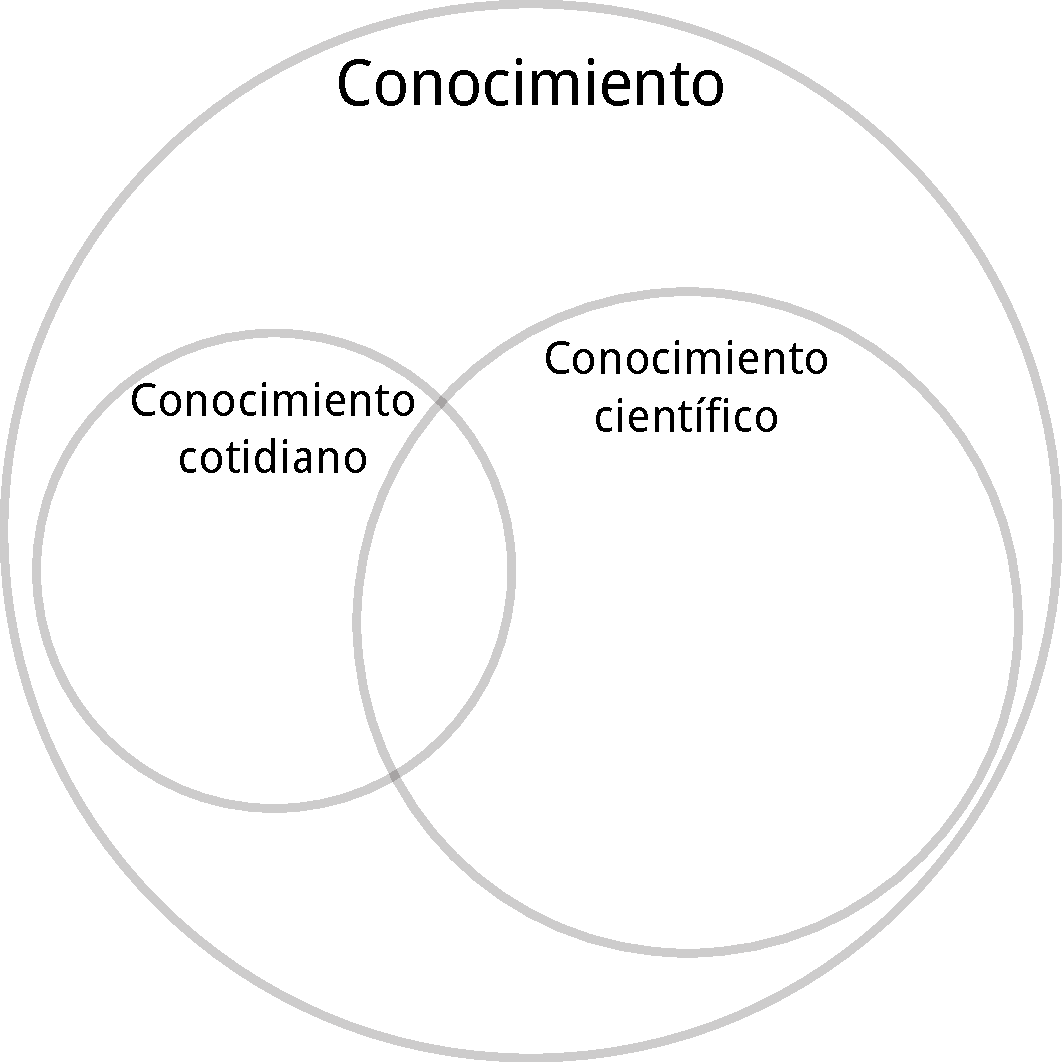
\includegraphics[height=18em]{venn.pdf}
      \end{center}
    \end{column}
  \end{columns}
\end{frame}

\begin{frame}{Ejemplares}
  \protect\phantomsection\label{ejemplares}
  ¿Qué ciencias son ejemplares canónicas de «ciencias»?

  \begin{columns}[T,onlytextwidth]
    \begin{column}{0.48\linewidth}
      \textbf{Ciencias}

      \begin{itemize}
          \tightlist
        \item
          Física
        \item
          Biología
        \item
          Química
      \end{itemize}
    \end{column}

    \begin{column}{0.48\linewidth}
      \textbf{No ciencias} (?)

      \begin{itemize}
          \tightlist
        \item
          Astrología
        \item
          Adivinación
        \item
          Homeopatía
      \end{itemize}
    \end{column}
  \end{columns}

  Hay otras disciplinas que son áreas grises.

  \begin{itemize}
      \tightlist
    \item
      Ciencias sociales
    \item
      Psicología
    \item
      Humanidades
  \end{itemize}
\end{frame}

\begin{frame}{El problema de la demarcación}
  \protect\phantomsection\label{el-problema-de-la-demarcaciuxf3n}
  La pregunta por distinguir \textbf{ciencia} de \textbf{no-ciencia} (o
  \emph{pseudociencia}) es conocido como el \textbf{problema de la
  demarcación}.

  Si es posible demarcar entre ciencia y no-ciencia, debe haber algún
  \textbf{criterio de demarcación}.

  Criterios tradicionales de demarcación:

  \begin{itemize}
      \tightlist
    \item
      Método científico
    \item
      Verificación, confirmación
  \end{itemize}
\end{frame}

\begin{frame}{El problema de la demarcación}
  \protect\phantomsection\label{el-problema-de-la-demarcaciuxf3n-1}
  \begin{block}{Método científico}
    \protect\phantomsection\label{muxe9todo-cientuxedfico}
    Se dice que la ciencia se identifica por el uso de un \textbf{método
    científico}.

    \begin{center}
      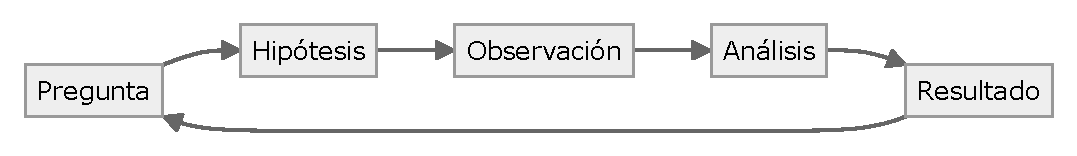
\includegraphics[width=40em]{fig1.pdf}
    \end{center}

    ¿De dónde sale la idea de que hay \emph{un} ``método científico''?

    ¿Siguen \emph{todas} las ciencias, y únicamente las ciencias, este
    método?
  \end{block}
\end{frame}

\begin{frame}{El problema de la demarcación}
  \protect\phantomsection\label{el-problema-de-la-demarcaciuxf3n-2}
  \begin{block}{Método científico}
    \protect\phantomsection\label{muxe9todo-cientuxedfico-1}
    Varias disciplinas ``pseudocientíficas'' cumplen con el uso de métodos
    similares:

    \begin{center}
      \begin{minipage}{0.9\textwidth}
        \begin{exampleblock}{Ejemplo}

          Pregunta: ¿Qué rasgos de la personalidad tienen las
          personas nacidas en agosto?\\
          Hipótesis: Tienden a ser entusiastas y creativas \\
          Observación: Algunas personas nacidas en agosto son
          entusiastas y creativas  \\
          Análisis: La observación concuerda con la hipótesis  \\
          Resultado: La hipótesis es verdadera  \\

        \end{exampleblock}
      \end{minipage}
    \end{center}
  \end{block}
\end{frame}

\begin{frame}{El problema de la demarcación}
  \protect\phantomsection\label{el-problema-de-la-demarcaciuxf3n-3}
  \begin{block}{Método científico}
    \protect\phantomsection\label{muxe9todo-cientuxedfico-2}
    Adicionalmente, algunos elementos de las ciencias paradigmáticas no
    siguen este método.

    \begin{quote}
      ``Todo cuerpo persevera en su estado de reposo o movimiento uniforme y
      rectilíneo a no ser que sea obligado a cambiar su estado por fuerzas
      impresas sobre él.''
    \end{quote}

    \vspace{0.5em}

    Es imposible obtener un sistema experimental sin ninguna
    fuerza.\vspace{0.5em}

    \textbf{Consecuencia:} Es imposible confirmar experimentalmente la
    primera ley de Newton.
  \end{block}
\end{frame}

\begin{frame}{El problema de la demarcación}
  \protect\phantomsection\label{el-problema-de-la-demarcaciuxf3n-4}
  \begin{block}{Verificación y confirmación}
    \protect\phantomsection\label{verificaciuxf3n-y-confirmaciuxf3n}
    Podríamos pensar que la ciencia se identifica por solo creer enunciados
    \textbf{bien confirmados} (i.e., con buena evidencia en su
    favor).\vspace{0.5em}

    Algunos problemas:

    \begin{enumerate}
        \tightlist
      \item
        Toda la evidencia posible confirma hipótesis triviales (e.g., ``Los
        capricornio son caprichosos o no lo son'').
      \item
        Con frecuencia creemos hipótesis antes de que haya evidencia en su
        favor (e.g., la relatividad no tenía todavía más evidencia en su favor
        que las teorías anteriores).
      \item
        Podemos interpretar la evidencia a favor de casi cualquier hipótesis
        (e.g., epiciclos)
    \end{enumerate}
  \end{block}
\end{frame}

\begin{frame}{El problema de la demarcación}
  \protect\phantomsection\label{el-problema-de-la-demarcaciuxf3n-5}
  \begin{block}{¿Dónde está el problema?}
    \protect\phantomsection\label{duxf3nde-estuxe1-el-problema}
    Con todo, parte del problema parece estar en la relación que hay entre
    los \textbf{hechos} y nuestras \textbf{teorías}.

    \begin{columns}[T,onlytextwidth]
      \begin{column}{0.48\linewidth}
        \begin{itemize}
            \tightlist
          \item
            Las teorías parecen contener expectativas sobre los hechos.
          \item
            Los hechos parecen confirmar y falsear teorías.
          \item
            Necesitamos confrontar los hechos para saber cuáles teorías son
            verdaderas y cuáles son falsas.
        \end{itemize}
      \end{column}

      \begin{column}{0.48\linewidth}
        Esto invita a algunas preguntas:

        \begin{itemize}
            \tightlist
          \item
            ¿Qué son los \textbf{hechos}?
          \item
            ¿Qué son las \textbf{teorías}?
          \item
            ¿Cuál es su conexión? ¿Podemos revisar hechos sin teoría?
        \end{itemize}
      \end{column}
    \end{columns}
  \end{block}
\end{frame}

\section{Problemas de filosofía de la
ciencia}\label{problemas-de-filosofuxeda-de-la-ciencia}

\begin{frame}{Ciencia y hechos}
  \protect\phantomsection\label{ciencia-y-hechos}
  ¿En qué sentido las teorías científicas dependen de los hechos?
  \vspace{-1em}

  \begin{columns}[T,onlytextwidth]
    \begin{column}{0.3\linewidth}
      \begin{block}{Confirmación}
        \protect\phantomsection\label{confirmaciuxf3n}
        ¿Cuándo decimos que los hechos \emph{confirman} una hipótesis?
      \end{block}
    \end{column}

    \begin{column}{0.3\linewidth}
      \begin{block}{Falsación}
        \protect\phantomsection\label{falsaciuxf3n}
        ¿Cuándo decimos que una hipótesis es \emph{falseada} por los hechos?
      \end{block}
    \end{column}

    \begin{column}{0.3\linewidth}
      \begin{block}{Subdeterminación}
        \protect\phantomsection\label{subdeterminaciuxf3n}
        ¿Cómo escogemos entre hipótesis \emph{compatibles} con los hechos?
      \end{block}
    \end{column}
  \end{columns}

  Para acercarnos a estas preguntas, estudiaremos:

  \begin{itemize}
      \tightlist
    \item
      El problema de la inducción
    \item
      El falsacionismo de Popper
    \item
      La tesis Duhem/Quine y los argumentos de subdeterminación empírica
  \end{itemize}
\end{frame}

\begin{frame}{Explicación científica}
  \protect\phantomsection\label{explicaciuxf3n-cientuxedfica}
  ¿Qué significa que la ciencia \emph{explique} un fenómeno? \vspace{-1em}

  \begin{columns}[T,onlytextwidth]
    \begin{column}{0.48\linewidth}
      \begin{block}{Modelo nomológico-deductivo}
        \protect\phantomsection\label{modelo-nomoluxf3gico-deductivo}
        Explicar un fenómeno es subsumirlo bajo una ley.

        \begin{itemize}
            \tightlist
          \item
            ¿Qué son las \emph{leyes} científicas?
          \item
            ¿Cuál es la relación lógica entre hechos y leyes?
        \end{itemize}
      \end{block}
    \end{column}

    \begin{column}{0.48\linewidth}
      \begin{block}{Modelo mecanicista}
        \protect\phantomsection\label{modelo-mecanicista}
        Explicar un fenómeno es encontrar el mecanismo que lo produce.

        \begin{itemize}
            \tightlist
          \item
            ¿Cuándo la explicación no requiere \emph{leyes}?
          \item
            ¿Qué es un mecanismo?
        \end{itemize}
      \end{block}
    \end{column}
  \end{columns}
\end{frame}

\begin{frame}{Ciencia, historia y progreso}
  \protect\phantomsection\label{ciencia-historia-y-progreso}
  ¿En qué sentido la ciencia \emph{progresa}? ¿Cómo debemos contar la
  \emph{historia} de la ciencia? \vspace{-1em}

  \begin{columns}[T,onlytextwidth]
    \begin{column}{0.3\linewidth}
      \begin{block}{Kuhn}
        \protect\phantomsection\label{kuhn}
        La ciencia progresa mediante \textbf{cambios de paradigma}.
      \end{block}
    \end{column}

    \begin{column}{0.3\linewidth}
      \begin{block}{Lakatos}
        \protect\phantomsection\label{lakatos}
        La ciencia progresa \textbf{falseando} teorías de manera no arbitraria.
      \end{block}
    \end{column}

    \begin{column}{0.3\linewidth}
      \begin{block}{Feyerabend}
        \protect\phantomsection\label{feyerabend}
        La ciencia progresa \textbf{rompiendo normas} aceptadas.
      \end{block}
    \end{column}
  \end{columns}

  \vspace{1em}

  También estudiaremos cómo la historia de la ciencia debe
  \emph{revaluarse} a la luz de sus sesgos (e.g., sesgos de género)
  (Harding).
\end{frame}

\section{Plan del curso}\label{plan-del-curso}

\begin{frame}{Objetivos de aprendizaje}
  \protect\phantomsection\label{objetivos-de-aprendizaje}
  \begin{enumerate}
      \tightlist
    \item
      Analizar la estructura lógica del problema de la inducción y algunas
      de sus consecuencias sobre la relación entre \textbf{hechos} y
      \textbf{ciencia}.
    \item
      Analizar la estructura e inferir algunas consecuencias de la tesis
      Duhem-Quine y los argumentos de \textbf{subdeterminación empírica}
      para la filosofía de la ciencia contemporánea y otras áreas de la
      filosofía.
    \item
      Comparar y contrastar los postulados centrales del modelo
      nomológico-deductivo y el modelo mecanicista de \textbf{explicación}.
    \item
      Distinguir las tesis principales y los argumentos centrales de algunos
      marcos filosóficos en la \textbf{historiografía} de la ciencia.
  \end{enumerate}
\end{frame}

\begin{frame}{Contenidos}
  \protect\phantomsection\label{contenidos}
  \begin{block}{Unidades}
    \protect\phantomsection\label{unidades}
    \begin{enumerate}
        \tightlist
      \item
        Ciencia y hechos

        \begin{enumerate}
            \setcounter{enumii}{2}
            \tightlist
          \item
            El (nuevo) problema de la \emph{inducción}
          \item
            El \emph{falsacionismo} de Popper
          \item
            \emph{Subdeterminación} empírica
        \end{enumerate}
      \item
        Explicación científica

        \begin{enumerate}
            \tightlist
          \item
            Modelo nomológico-deductivo
          \item
            Modelo mecanicista
        \end{enumerate}
      \item
        Ciencia, historia y progreso

        \begin{enumerate}
            \tightlist
          \item
            Kuhn y la noción de \emph{paradigma}
          \item
            El \emph{falsacionismo sofisticado} de Lakatos
          \item
            Feyerabend y el anarquismo epistemológico
          \item
            Harding y el feminismo en historiografía de la ciencia
        \end{enumerate}
    \end{enumerate}
  \end{block}
\end{frame}

\begin{frame}{Evaluaciones}
  \protect\phantomsection\label{evaluaciones}
  \begin{columns}[T,onlytextwidth]
    \begin{column}{0.3\linewidth}
      \begin{block}{Taller de lógica (30\%)}
        \protect\phantomsection\label{taller-de-luxf3gica-30}
        Taller \textbf{asincrónico} sobre lógica formal (repaso) y epistemología
        de las ciencias.

        \begin{itemize}
            \tightlist
          \item
            No requiere conocimientos previos.
        \end{itemize}

        \textbf{Fecha:} 2 de septiembre
      \end{block}
    \end{column}

    \begin{column}{0.3\linewidth}
      \begin{block}{Examen presencial (30\%)}
        \protect\phantomsection\label{examen-presencial-30}
        Examen \textbf{presencial} sobre inducción y subdeterminación empírica.

        \textbf{Fecha:} 7 de octubre
      \end{block}
    \end{column}

    \begin{column}{0.3\linewidth}
      \begin{block}{Examen pedagógico (40\%)}
        \protect\phantomsection\label{examen-pedaguxf3gico-40}
        Microlección asincrónica para estudiantes de nivel escolar.

        \textbf{Fecha:} 25 de noviembre
      \end{block}
    \end{column}
  \end{columns}
\end{frame}

\begin{frame}{Reglas de juego}
  \protect\phantomsection\label{reglas-de-juego}
  \begin{block}{Correcciones}
    \protect\phantomsection\label{correcciones}
    Será posible entregar \textbf{correcciones} del \textbf{taller} y el
    \textbf{examen}.

    Se comunicará una \textbf{guía de corrección} con anterioridad.

    Se evalúa:

    \begin{itemize}
        \tightlist
      \item
        Corrección (50\%)
      \item
        Explicación y reflexión sobre la corrección (50\%)
    \end{itemize}

    Se podrá entregar \textbf{una semana} después de \textbf{recibir}
    retroalimentación.
  \end{block}
\end{frame}

\begin{frame}{Asistencia}
  \protect\phantomsection\label{asistencia}
  La asistencia es \textbf{obligatoria} y responsabilidad de cada
  estudiante.

  Es necesario asistir a mínimo \textbf{70\%} de las sesiones de clase
  para aprobar el curso.

  \begin{columns}[T,onlytextwidth]
    \begin{column}{0.48\linewidth}
      Si hay inasistencia justificada:

      \begin{itemize}
          \tightlist
        \item
          Presenten su excusa según el Reglamento Académico.
      \end{itemize}
    \end{column}

    \begin{column}{0.48\linewidth}
      Si hay inasistencia reglamentariamente injustificada:

      \begin{itemize}
          \tightlist
        \item
          ¡Hablen conmigo!
        \item
          Podemos negociar fechas, entregas, etc.
      \end{itemize}
    \end{column}
  \end{columns}
\end{frame}

\begin{frame}{Sobre el plagio}
  \protect\phantomsection\label{sobre-el-plagio}
  Cometer plagio no solo es moralmente condenable, sino poco inteligente.

  \begin{itemize}
      \tightlist
    \item
      Pagan por aprender, pero entorpecen su propio aprendizaje.
    \item
      Engañan al profesor a pensar que han aprendido más de lo que realmente
      han aprendido.
    \item
      Impiden el desarrollo orgánico de la clase, obstaculizando el
      aprendizaje de sus colegas.
  \end{itemize}

  Cualquier plagio detectado será reportado según el Reglamento Académico.

  El profesor puede \textbf{solicitar} material adicional en cualquier
  evaluación.
\end{frame}

\begin{frame}{Comunicaciones}
  \protect\phantomsection\label{comunicaciones}
  Toda la comunicación será mediante el \textbf{correo institucional} o
  mediante \textbf{UCampus}. \vspace{-1em}

  \begin{center}
    \begin{minipage}{0.9\textwidth}

      \begin{alertblock}{¿Y qué pasa si no funciona mi correo institucional?}

        ¡Busque inmediatamente que funcione!

        Ese es el mecanismo de comunicación oficial con la
        universidad, incluyendo este curso.

        Sin ese mecanismo, es como si no tuvieran internet,
        computador, etc. (i.e., son condiciones necesarias para la
        comunicación.)

      \end{alertblock}
    \end{minipage}
  \end{center}

  Podrán contactarme a \textbf{jloaiza@uahurtado.cl}.
\end{frame}

% Bibliography slide

\end{document}
